\documentclass{article}

\usepackage{amsmath,amsfonts,amssymb}   

\newif\ifanswer
%\answertrue
\answerfalse

\let\imp=\Rightarrow
\let\iff=\Leftrightarrow
\usepackage{graphicx}
\usepackage{listings}
\usepackage{tikz-qtree}
\lstset{language=C}


\tikzset{every tree node/.style={minimum width=2em,draw,circle},
         blank/.style={draw=none},
         edge from parent/.style=
         {draw,->, edge from parent path={(\tikzparentnode) -- (\tikzchildnode)}},
         level distance=1.5cm}

\begin{document}

\section*{COMS10011 sample paper}

THIS IS STILL A WORK IN PROGRESS but is close to its final form! This
is a sample paper, it has the same style of question as the real
paper, the layout is slightly different in trivial ways to the
official exam layout.

\subsection*{Rubric}{
This paper contains \emph{two} parts. \\
The first section contains \emph {15} short questions.\\ 
Each question is worth \emph{two marks} and all should be attempted.\\
The second section contains \emph {three} long questions.\\
Each long question is worth \emph{20 marks}.\\
The best \emph{two} long question answers will be used for assessment. \\
The maximum for this paper is \emph{70 marks}. \\
Calculators must have the Faculty of Engineering Seal of Approval.}

%MSM: unit specific Latex commands 

\subsection*{Section A: short questions - answer all questions}

\begin{enumerate}

%1 conor
\item What is the definition of Shannon's entropy for a discrete distribution?

  \ifanswer \textbf{Answer}:\\
  For sample space $\mathcal{X}$ we have
  \begin{equation}
    H(X)=-\sum_{x\in\mathcal{X}}p(x)\log{p(x)}
  \end{equation}
  \fi

  %2 conor

\item If you have a finite set of $n$ spike trains and calculate the
  entropy of the spike trains using the discretization method proposed
  by Bialek and co-workers, in general, what limit would the entropy
  reach as the time step is made very small?

  \ifanswer \textbf{Answer}:\\ If the time step is small enough each spike train would
  correspond to a different word, with small enough time step, each
  spike in each train would, in general, fall into a different time
  bins. This means there would be $n$ different words, each with one
  occurance and hence probability $1/n$. Thus the entropy would be
  $\log{n}$. I recently had to reject a paper where the authors had
  completely misunderstood this!
  \fi
  
%3 conor
\item Given a Markov chain $V\rightarrow X\rightarrow H$ what can we say about $p_{V,H|X}(v,h|x)$?

\ifanswer \textbf{Answer}:\\
\begin{equation}
p_{V,H|X}(v,h|x)=p_{V|X}(v|x)p_{H|X}(h|x)
\end{equation}
\fi
%4 conor
\item What is the cocktail party problem?

  \ifanswer \textbf{Answer}:\\ Often the environment is very noisy with a sound, such as a voice, that is being attended to, not much distinguished in amplitude from other noises. I have read that this situation holds at \lq{}cocktail parties\rq{}, a form of social entertainment popular in the last century somewhat akin to pre-drinks but without going anywhere afterwards. The cocktail party problem is the question of how the brain separates the sound signal it is attending to from the background noise.
  \fi

%5 conor
\item In the Eriksen flanker task sketch the accuracy versus
reaction time for the consistent, \textbf{HHH}, and inconsistent,
\textbf{HSH}, conditions. The overall scale of the reaction time is
not what is being asked for, rather the shape.

\ifanswer \textbf{Answer}:\\
In both cases the line starts at 0.5 but in the consistent case it
rises quickly to one, in the inconsistent case it falls below 0.5
before rising more slowly to one. [1 mark for starting at 0.5 and rising to 1, the other for the dip in inconsistent].
\fi

%6 conor
\item The $n$-armed bandit task is used in psychological studies of decision making. What is an $n$-armed bandit?

  \ifanswer \textbf{Answer}:\\
  In an $n$-armed bandit the participant has to chose between $n$ options, typically $n$ buttons, each with a different probability of reward.
  \fi

  %7 conor
\item If four options in a decision task have estimated reward values $r_1$, $r_2$, $r_3$ and $r_4$, what is the soft-max probability for chosing the $i$th option?

  \ifanswer \textbf{Answer}:\\
  \begin{equation}
    p_i=\frac{e^{\beta r_i}}{\sum_j e^{\beta r_j}}
  \end{equation}
  for some $\beta$, a parameter determining the exploration to exploitation balance.
  \fi


  %1 rui
\item Define the credit assignment problem in neuroscience.

  \ifanswer \textbf{Answer}: The credit assignment is the problem of deciding how to change parameters in the brain (typically synaptic weights) to best improve behaviour (e.g. a desired motor output).
  \fi
  
    %2 rui
\item What are the two key features of gated recurrent neural networks?

  \ifanswer \textbf{Answer}: Gated RNNs have two defining features, the memory cell and the gating units.\\
  \fi
  
     %3 rui
\item What is the key difference between supervised and reinforcement learning in terms of their cost function?

  \ifanswer \textbf{Answer}: The existence of a teacher (or teaching signal) in supervised learning, and a reward signal in reinforcement learning.\\
  \fi
  
  
     %4 rui
\item What types of features are learned by sparse coding algorithms when applied to natural images?

  \ifanswer \textbf{Answer}: Features representing statistics of natural images, such as oriented bars/edges.\\
  \fi
  
     %5 rui
\item Give the classical cost function used in sparse coding.

  \ifanswer \textbf{Answer}: $\mathrm{cost} = \Vert U - WV \Vert_2^2 + \lambda \Vert V\Vert_1$, where $V$ is the activity of output neurons and $U$ is the input activity of input neurons. The second term enforces sparsity.\\
  \fi
  
     %6 rui
\item Give the value update function used in Q-Learning? How does it differ from TD learning?

  \ifanswer \textbf{Answer}: $\underbrace{Q(S_t, A_t)}_{\mathrm{value}} = Q(S_t, A_t) + (\overbrace{\underbrace{R_{t+1}}_{\mathrm{reward}}+\lambda \underbrace{\mathrm{max}_a Q(S_{t+1},a)}_{\mathrm{future\:value}}}^{\mathrm{learned\:value}}-Q_{t}(S_t,A_t))$. It differs from TD learning in that it takes the action with maximal value for the update, which makes Q-learning an off-policy method.\\
  \fi

  %1 cian
\item How many different joint activity patterns could a population of $N$ binary neurons generate? Why is it often hard to estimate the probability distribution across these patterns from neural population data?

\ifanswer \textbf{Answer:} There are $2^N$ possible binary patterns (1 mark). Estimation is hard because $2^N$ is a very large number for any reasonable sized number of neurons, say $N\gtrapprox 20$. In contrast, a typical neural recording may only be about an hour, which would correspond to only $3.6\times10^5$ time bins of $10$ ms each (1 mark for something similar to this reasoning).\\
\fi
  
  %2 cian
\item What is the basic idea underlying the dichotomised Gaussian model for neural population data?

  \ifanswer \textbf{Answer:} This model assumes that our observed binary data (spike patterns across the population of neurons) was generated by thresholding an underlying latent (hidden) multivariate gaussian distribution.
  \fi

\end{enumerate}
  
\section*{Section B: long questions - answer two questions}

\begin{enumerate}

%question from conor
\item This question is about the Kalman filter. 
\begin{enumerate}
\item{}[7 marks] Consider two random variables which are conditionally independent with normal distributions:
  \begin{eqnarray}
    p_{X|H}(x|h)&=&\frac{1}{\sqrt{2\pi\sigma_X^2}}e^{-(x-h)^2/2\sigma_X^2}\cr
    p_{Y|H}(y|h)&=&\frac{1}{\sqrt{2\pi\sigma_Y^2}}e^{-(y-h)^2/2\sigma_Y^2}
  \end{eqnarray}
  then $p_{X|H}(x|h)p_{Y|H}(y|h)$ is proportional to a normal distribution in $h$. What is that normal distribution?
 
  \ifanswer \textbf{Answer}:\\  Well this is just an exercise in matching terms, with the obvious notation:
  \begin{equation}
    \frac{1}{\sigma^2}(h^2-2h\mu)=\frac{1}{\sigma_X^2}(h^2-2hx)+\frac{1}{\sigma_Y^2}(h^2-2hy)
  \end{equation}
  so
  \begin{equation}
    \frac{1}{\sigma^2}=\frac{1}{\sigma_X^2}+\frac{1}{\sigma_Y^2}
  \end{equation}
  and
  \begin{equation}
  \mu=\frac{\sigma^2}{\sigma_X^2}x+\frac{\sigma^2}{\sigma_Y^2}y
  \end{equation}
  \fi
\item{}[8 marks] Consider an object moving at constant speed $v$ so that its position $x$ after a time $\delta t$ is
  $$
  x(t+\delta t)=x(t)+v\delta t+\xi
  $$ where $\xi$ is random noise drawn from
  $\mathcal{N}(0,\sigma^2_s)$. A sensor estimates the position of the
  object with noise drawn from $\mathcal{N}(0,\sigma^2_s)$. Derive the
  Kalman gain for optimally estimating the position of the object.

  \ifanswer \textbf{Answer}:\\ Let $h(t)$ be the estimated position with uncertainty
  $\sigma_h^2(t)$, after $\delta t$ the dead reckoning estimate is
  $d=h+v\delta t$ with uncertainty given by variance
  $\sigma_d^2=\sigma_h^2+\sigma_s^2$. Then we do Bayesian fusion to calculate the new estimated position
 
  \begin{equation}
    h(t+\delta t)=\frac{\sigma_h^2(t+\delta t)}{\sigma_d^2} d+\frac{\sigma_h^2(t+\delta t)}{\sigma_s^2} s
  \end{equation}
  where $s$ is the sensor estimate and
  \begin{equation}
    \frac{1}{\sigma_h^2(t+\delta t)}=\frac{1}{\sigma_d^2}+\frac{1}{\sigma_s^2}
  \end{equation}
  Rearranging this gives
  \begin{equation}
    h(t+\delta t)=d+k(s-d)
  \end{equation}
  where
  \begin{equation}
    k=\frac{\sigma_h^2(t+\delta t)}{\sigma_s^2}=\frac{\sigma_d^2}{\sigma_d^2+\sigma_s^2}
  \end{equation}
  This is the same calculation done in the Kalman filter notes, just with a slightly different notation.
\fi
  
\item{}[5 marks] Explain what is meant by a forward model for motor control.

  \ifanswer \textbf{Answer}:\\ In a forward model the brain predicts the effect of a
  motor command, this is used to calculate the next motor command is a
  feedback control loop; sensor feedback is used to correct the
  prediction. For movement the prediction will be a dead reckoning estimate.
  \fi
  
  \end{enumerate}
  
%question split between conor and cian  
\item There are two parts to this question, the first is about information theory, the second is about statistical models.
  \begin{enumerate}
  \item{Information theory}
\begin{enumerate}
\item{}[3 marks] Define $I(X;Y)$ and give a sufficient condition for $I(X;Y)=0$ for non-trivial random variables $X$ and $Y$?
  \ifanswer \textbf{Answer}:\\
  \begin{equation}
  I(X;Y)=\sum_{x,y}p(x,y)\log{\frac{p(x,y)}{p(x)p(y)}}
  \end{equation}
  and this is zero if the argument of the log is zero, that is $p(x,y)=p(x)p(y)$ for all $x$ and $y$, that is when $X$ and $Y$ are independent.
  \fi
\item{}[4 marks]
 Calculate the mutual information between random variables $X$ and $Y$ with sample spaces $\mathcal{X}=\{\mbox{a},\mbox{b},\mbox{c}\}$ and $\mathcal{Y}=\{\alpha,\beta\}$.
  \begin{center}
  \begin{tabular}{c|ccc}
    \hline
    &\mbox{a}&\mbox{b}&\mbox{c}\\
    $\alpha$&0.5&0.125&0\\
    $\beta$&0&0.125&0.25
    \end{tabular}
  \end{center}
You can write the answer in terms of $\log{3}$ and $\log{5}$ if you would prefer.
  
  \ifanswer \textbf{Answer}:\\
So to marginalize we have, using the obvious abuse of notation $p(X)=\{0.5,0.25,0.25\}$ and $p(Y)=\{0.625,0.375\}$ so the table for $p_X(x)p_Y(y)$ is
  \begin{center}
  \begin{tabular}{c|ccc}
    \hline
    &\mbox{a}&\mbox{b}&\mbox{c}\\
    $\alpha$&5/16&5/32&5/32\\
    $\beta$&3/16&3/32&3/32
    \end{tabular}
  \end{center}
  now
  \begin{equation}
    I(X;Y)=\sum_{x,y}p(x,y)\log{\frac{p(x,y)}{p(x)p(y)}}
  \end{equation}
  so
  \begin{eqnarray}
    I(X;Y)&=&\frac{1}{2}\log{\frac{1/2}{5/16}}+\frac{1}{4}\log{\frac{1/8}{5/32}}+\frac{1/4}\log{\frac{1/8}{3/32}}+\frac{1}{4}\log{\frac{1/4}{3/32}}\cr
    &=&\frac{1}{2}\log{\frac{8}{5}}+\frac{1}{4}\log{\frac{4}{5}}+\frac{1/4}\log{\frac{4}{3}}+\frac{1}{4}\log{\frac{8}{3}}\cr
    &=&\frac{13}{4}-\frac{3}{4}\log{5}-\frac{1}{2}\log{3}\approx 0.716
  \end{eqnarray}

  \fi

\item{}[3 marks] Show $I(X;Y)=H(X)-H(X|Y)$.

  \ifanswer \textbf{Answer}:\\
  So we start with the definition of the mutual information
  \begin{equation}
    I(X;Y)=\sum_{x,y} p(x,y)\log{\frac{p(x,y)}{p(x)p(y)}}
  \end{equation}
  and then write $p(x,y)=p(x|y)p(y)$ giving
    \begin{eqnarray}
    I(X;Y)&=&\sum_{x,y} p(x,y)\log{\frac{p(x|y)}{p(x)}}\cr &=&\sum_{x,y}p(x,y)\log{p(x|y)}-\sum_{x,y}p(x,y)\log{p(x)}
  \end{eqnarray}
In the first term write $p(x,y)=p(x|y)p(y)$ again to get the definition of $H(X|Y)$ and in the second term sum over $y$ to marginalize $p(x,y)$ to $p(x)$.
  \fi
\end{enumerate}
\item Statistical models.\\

The pairwise and K-pairwise maximum entropy statistical models are often used for neural population data. The K-pairwise model gives the probability for a neural population activity pattern as 

$$
p(x_1,x_2,\ldots,x_N) = \frac{1}{Z}\exp[\sum_i h_i x_i + \sum_{i \neq j} J_{ij} x_i x_j + V(\sum_i x_i)]
$$

  
\begin{enumerate}

\item{}[3 marks] The equation for the standard pairwise maximum entropy model differs from the above by one term. Which term does it omit? 

\ifanswer \textbf{Answer:} The third term on the right hand side $V(\sum_i x_i)$ is omitted from the pairwise model. \fi

\item{}[6 marks] How many unique parameters do each of the pairwise and K-pairwise maximum entropy models have?

\ifanswer \textbf{Answer:} The pairwise model has $N + \frac{N(N-1)}{2}$ parameters, the K-pairwise model has  $N + \frac{N(N-1)}{2} + N + 1$ parameters. In each case the first $N$ parameters correspond to each of the individual neuron biases, the $h_i$'s. The second set of parameters are the pairwise couplings, $J_{ij}$'s. There is one of these for every possible pair of neurons. The division by two is because the couplings are symmetric, so $J_{ij}=J_{ji}$. And the K-pairwise model has a further $N+1$ parameters, one for each of the possible numbers of neurons simultaneously active, $k=0, k=1, k=2,\ldots,k=N$. [3 marks for each case. In both cases partial marks will be awarded for an approximately right answer that provides some reasoning.] \fi

\item{}[1 mark]  Which of the two models more accurately matches neural population data? [1 mark]

\ifanswer \textbf{Answer:} The K-pairwise model more accurately matches the data: it captures some higher-order correlations. Also, since the pairwise model is a special case of the K-pairwise (where all the $V$ terms equal zero), then the K-pairwise model must only do at least as well as or better than the pairwise model.\fi
  
\end{enumerate}

  \end{enumerate}


%question from rui
\item This question is about supervised learning in the brain.
\begin{enumerate}
\item{}[5 marks] How may the brain implement supervised learning?

  \ifanswer \textbf{Answer}: The classical example of supervised learning in the brain is in the cerebellum, where specific error signals appears to be computed [2.5 marks]. However, the cortex may also use some forms of supervised learning by relying on internally generated supervised signals, which may in turn use algorithms akin to the backpropagation algorithm to efficiently update synaptic weights [2.5 marks].\\
  \fi


\item{}[11 marks] Give one feature that has been suggested to make the backpropagation algorithm used in supervised learning biologically implausible? You should use a simple two layer neural network (with one hidden neuron $h$, one output neuron $v$, one input weights, and no biases, see Figure~\ref{fig:backprop_ff}) to derive the weight update. Assume the cost function (or error) to be $E = (v-y)^2$, where $y$ is the desired target.

\begin{figure}[htb!]
  \centering
  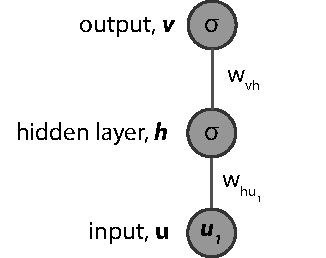
\includegraphics[width=0.4\linewidth]{backprop_ff}
  \caption{\textbf{Schematic of simple feedfoward neural network, with quadratic units $\sigma (x) = x^2$.}}
  \label{fig:backprop_ff}
\end{figure}

  \ifanswer \textbf{Answer}: To illustrate the backprop algorithm we provide the update rule for weight $w_{hu_1}$ (similar for $w_{hu_2}$) is given by $\frac{\partial E}{\partial w_{hu_1}} = \frac{\partial E}{\partial v}\frac{\partial v}{\partial h}\frac{\partial h}{\partial w_{hu_1}}$ [1 mark]. For the network considered here, these components are [1 mark for each]:
\begin{equation}
\frac{\partial E}{\partial v} = 2(v-y)
\label{eq:dEdv}
\end{equation}
\begin{equation}
\frac{\partial v}{\partial h} = \sigma'_v w_{vh}
\label{eq:dvdh}
\end{equation}
\begin{equation}
\frac{\partial h}{\partial w_{hu_1}} = \sigma'_h u_1
\label{eq:dhdw}
\end{equation}
which together yields $\frac{\partial E}{\partial w_{hu_1}} = 2(v-y) \sigma'_v w_{vh} \sigma'_h u_1$, where $\sigma'=2x$ denotes the derivative of the linear activation function [2 marks]. Note: A good exercise is to represent the different components of the gradient in the schematic of the network.\\


Any of the following features can be indicated [5 marks]\\
\begin{itemize}
\item \textit{Weight transport problem}: the existence os symmetric weights (i.e. feedback weights derived from backprop are equal to feedforward weights, e.g. $w_{vh}$ (as in Eq.~\ref{eq:dEdv}). Synaptic weights are unidirectional in the brain, which makes symmetric feedforward and feedback weights implausible.\\

\item \textit{Derivative of activation (input-output) function}: Backprop needs the derivative of the neuronal activation function (as in Eqs.~\ref{eq:dvdh} and \ref{eq:dhdw}), which is unclear how it is computed biologically.\\

\item \textit{Target or teaching signal}, unclear whether the brain could provide such a teaching signal needed for the cost/error function. However, in principle, different brain areas encoding different aspects of the environment can act as teachers of other brain areas, or such teaching signal could be provided by an external teacher.\\

\item \textit{Weight learning rule is non-local}: synaptic plasticity (i.e. modification of synaptic weights) typically depends only on locally available information (e.g. pre and postsynaptic activity). However, classical backprop relies on non-local information (error signal, as in $\frac{d E}{d w_{hu_1}}$).\\

\item \textit{Separate learning phase}: Learning needs its only separate phase. Backprop relies on first having a forward phase to update activity and then a backward phase to calculate the error and update the neural network parameters. There is no evidence of such a clear separation between activity and learning in neuroscience.\\

\item \textit{Separate error network}: The use of a separate learning phase with errors, suggests the need for a separate error network. There is no evidence for such separate error networks.\\
\end{itemize}
  \fi


\item{}[4 marks] What features do artificial neuronal networks trained with backprop learn (e.g. when trained to discriminate objects in images)? Why do they provide a good match to the activity of neurons in the brain? \\

  \ifanswer \textbf{Answer}: Artificial neural networks (ANNs) learn to detect features similar to the ones observed in the brain [1 mark], such as oriented bars or Gabor-like receptive fields, but also face-like features [1 mark]. Given that both ANNs and the brain need to be optimised to discriminate images [1 mark] and that there is recent evidence for learning principles similar to backprop in the brain [1 mark] this might explain why these networks are good computational models of neuronal data.\\
  \fi

\end{enumerate}  
 \end{enumerate}
 

\end{document}
